\section{Vorbereitung}
\label{sec:preperation}

\subsection{}
Wir haben den Ordner mit den Audiodateien wie vorgesehen eingebunden.
Der Pfad zu diesem Ordner lässt sich vom Nutzer einfach konfigurieren, indem der Pfad in Zeile 2 der main.m angepasst wird.

\subsection{}
Das Einbinden der Timbre Toolbox (TTB) erwies sich als wesentlich komplizierter als beschrieben.
Nach dem Einbinden des TTB Ordners in den Matlab Pfad, stellte sich heraus, dass der Code nicht mehr unterstützte Matlab Funktionen verwendet.
Um die TTB mit Matlab in der Version \texttt{R2016b} verwenden zu können, musste in der Datei \texttt{cSound.m} die Zeile 53 gegen folgende Zeilen ausgetauscht werden:

\begin{lstlisting}
[c.f_Sig_v, c.f_Fs] = audioread(c.w_FileName);
info                = audioinfo(c.w_FileName);
c.i_Bits            = int16(info.BitsPerSample);
\end{lstlisting}

Das Hinzufügen der Datei für den SWIPE-Algorithmus\footnote{\url{http://www.cise.ufl.edu/~acamacho/publications/swipep.m}} erwies sich als äußerst schwierig.
Wenn die Datei, wie in der Dokumentation beschrieben, in den Pfad \texttt{\$TTB\_ROOT\_DIR/classes/cHarmRep/} eingefügt wurde, fand Matlab die Funktion \texttt{swipep} selbst nach Einbinden der Datei in den Pfad nicht.
Nach langem Rumprobieren gelang es das Problem zu lösen, indem die Datei \texttt{swipep.m} aus dem \texttt{cHarmRep} Ordner ins Basisverzeichnis neben die \texttt{main.m} Datei verschoben wurde.

\section{Analyse}
\label{sec:analyse}

\subsection{}
Die Analyse lies sich problemlos durchführen.
Für jede Datei wurden 98 Deskriptoren errechnet.	
Der Parameter \texttt{config\_s.threshold\_harmo} wurde nach einigen Testdurchläufen auf \texttt{0.01} festgelegt, damit alle Dateien analysiert werden.
Die Matrizen der extrahierten Deskriptoren wurden für jede Datei einzeln im Verzeichnis \texttt{Features} gespeichert, um eine spätere Bearbeitung in Python zu ermöglichen. 


\subsection{}
Die Matlab Parallel Computing Toolbox ist in der Studenten Version \texttt{R2016b} nicht enthalten.
Die Installation der Toolbox kostet zusätzlich 20 Euro.
Während ein Durchlauf einer normalen \texttt{for} Schleife ca. 5 Minuten dauert, braucht die parallelisierte Version der \texttt{for} Schleife ca. 3 Minuten.
Beide Durchläufe wurden auf einem Dell XPS 13 Notebook mit einem 2.4 GHz Intel Core i5 Prozessor aus der Skylake Generation und 8 GB RAM ausgeführt.

Das Speichern der Matrizen mit Hilfe der Funktion \texttt{save} ist in Matlab innerhalb einer \texttt{parfor} Schleife nicht möglich.
Deshalb wurde die Speicherfunktionalität in die Funktion \texttt{saveToFile} ausgelagert.

\newpage

\section{Clustering}
\label{sec:cluster}

\textbf{Anmerkung:} Im dritten Aufgabenteil haben wir die extrahierten Audio-Features aus Aufgabenteil \ref{sec:analyse} mit Python weiter verarbeitet und grafisch aufbereitet.
Dafür wurde die Python Version 3.6.1 genutzt und über den Paketmanager \textit{Pip} folgende Pakete installiert: \textit{scipy, numpy, matplotlib, scikit-learn, glob}.
Als Entwicklungsumgebung kam \textit{PyCharm} von \textit{IntelliJ} zum Einsatz.

\subsection{}
\label{ssec:3a}
Da Musiker sich während des Spielens bewegen, und außerdem verschiedene Töne in unterschiedlicher Haltung spielen, kann es zu Variationen des Mikrofonabstands und vor allem auch des Winkels zwischen Mikrofon und Instrument kommen. 
Sowohl die Winkelabhängigkeit der Abstrahlcharakteristik der Violine, als auch die Richtcharakteristik des Mikrofons beeinflussen den vom Mikrofon detektierten absoluten Schalldruck, welcher in direktem Verhältnis zu den Leistungsgrößen steht. 
Diese Schwankungen sind verhältnismäßig klein, wenn die Violine in ein und demselben Raum mit konstanten Mikrofonabstand aufgenommen wird, haben aber einen Einfluss.
Des weiteren ist es sinnvoll Deskriptoren zu verwenden, die auch für Audiodateien aus verschiedenen Aufnahmesituationen funktionieren und somit in der absoluten Leistung, welche von der Raumimpulsantwort, vom Instrument, vom Mikrofon und vom Abstand der beiden Letzteren abhängt, nicht mehr vergleichbar sind.
Stattdessen können wir zur Klassifizierung der Dynamikstufen Deskriptoren verwenden, die auf den veränderten Klangcharakter aufgrund unterschiedlichem harmonischem Gehalt bzw. die spektrale Färbung laut oder leise gespielter Töne abzielen.
Außerdem macht es Sinn auch temporale Deskriptoren zu betrachten, die die Spielweise des Musikers beschreiben.
\subsection{}
Spielt man eine Violine mit mehr Dynamik, treten die Obertöne stärker hervor.
Wenn man also den Bogen schnell und mit viel Druck über die Saite streicht liefern die harmonischen Frequenzen, also die Vielfachen der Grundfrequenz, größere Energiebeiträge im Verhältnis zur Gesamtenergie, welche auch den Anteil inharmonischer bzw. geräuschhafter Anteile enthält.  
Ein harmonischer Deskriptor, der diesen Effekt gut beschreibt ist die \textit{Harmonic Energy}.
Sie gibt das Verhältnis der durch Partialtöne erklärten Energie zur Gesamtenergie an.
Da es sich um einen zeitabhängigen Deskriptor handelt, gibt uns die Timbre Toolbox den Median als einzelnen Wert für eine Audiodatei.\\ 
Derselbe Effekt lässt sich auch mithilfe eines spektralen Features beschreiben.
Die \textit{Spectral Skewness} beschreibt die Asymmetrie des Spektrums um den Spectral Centroid herum.
Wir erwarten hier auch unterschiedliche Werte, da aufgrund der angereicherten Obertöne bei lauter Spielweise ein stärkeres Gewicht bei hohen Frequenzen liegen sollte, also rechts vom Spectral centroid.
Da dieser Deskriptor ebenfalls zeitabhängig ist, betrachten wir wieder den Median.

Beim Spielen lauter Töne wird zudem der Ton schneller aufgebaut, was mit der Geschwindigkeit des Bogens zusammenhängt.
Außerdem wird der Bogen bei leise gespielten Tönen langsamer von der Saite genommen.
Diese beiden Merkmale lassen sich mit den temporalen Deskriptoren \textit{Attack Time} und \textit{Release Time} erfassen.

\subsection{}
Wir gehen davon aus, dass die analysierten Violinen-Audiodateien unter gleichbleibenden Aufnahmebedingungen entstanden sind. 
Deswegen sollte die Dynamikstufe mit der Leistung verknüpft sein, d.h. lauter Spielen gibt uns mehr Energie pro Zeiteinheit, wenn wir die in Abschnitt \ref{ssec:3a} beschriebenen Schwankungen außer Beracht lassen.
Wir verwenden deswegen die \textit{Frame Energy} als leistungsabhängiges Feature.

Beim Blick auf die Scatterplots (siehe Abbildungen \ref{fig:harmonic_energy} bis \ref{fig:release_time}) sehen wir allerdings nur beim Deskriptor Harmonic Energy eine deutliche Korrelation mit der Frame Energy. 
Dies hätten wir eigentlich auch bei den anderen leistungsunabhängigen Größen erwartet hätten, sofern wir die Frame Energy als direkten Indikator für Dynamik ansehen.
Die Harmonic Energy ist in unserem Fall also der geeignetste Deskriptor um Dynamikstufen zu klassifizieren.

\begin{figure}[H]
    \center
    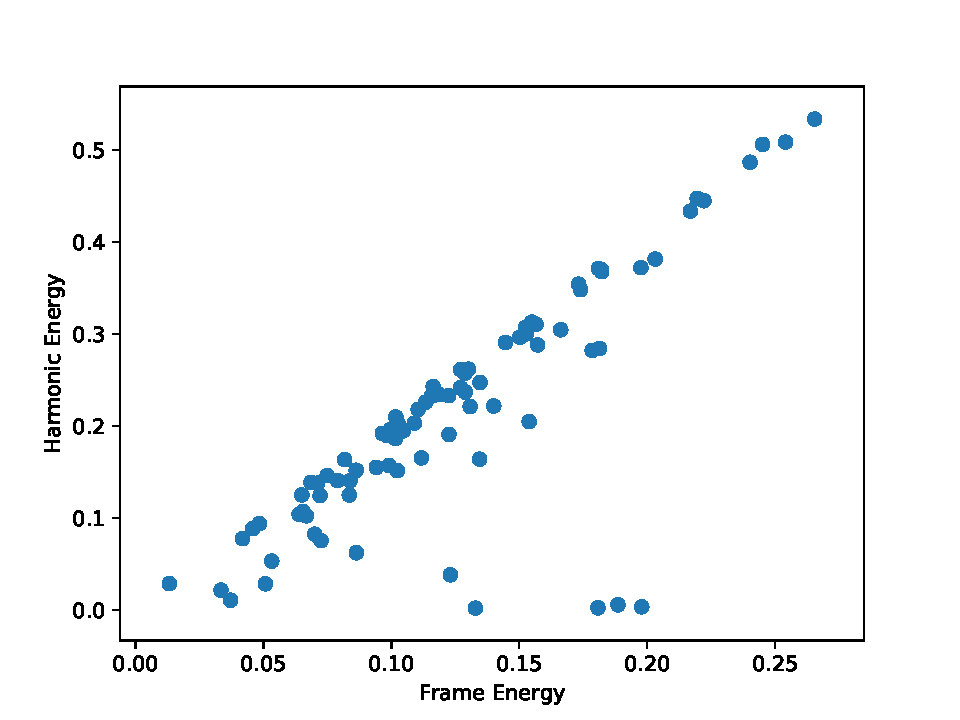
\includegraphics[width = 0.8\textwidth]{Figures/harmonicErg}
    \caption{Harmonic Energy über Frame Energy }
    \label{fig:harmonic_energy}
\end{figure}

\begin{figure}[H]
    \center
    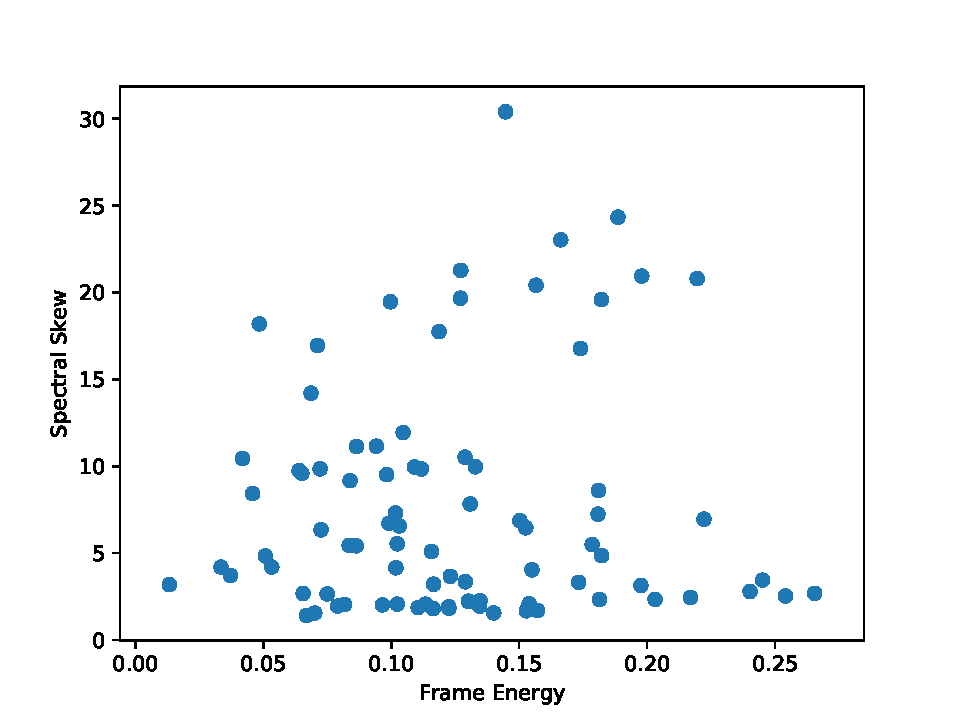
\includegraphics[width = 0.8\textwidth]{Figures/specSkew.pdf}
    \caption{Spectral Skew über Frame Energy}
    \label{fig:spectral_skew}
\end{figure}

\begin{figure}[H]
    \center
    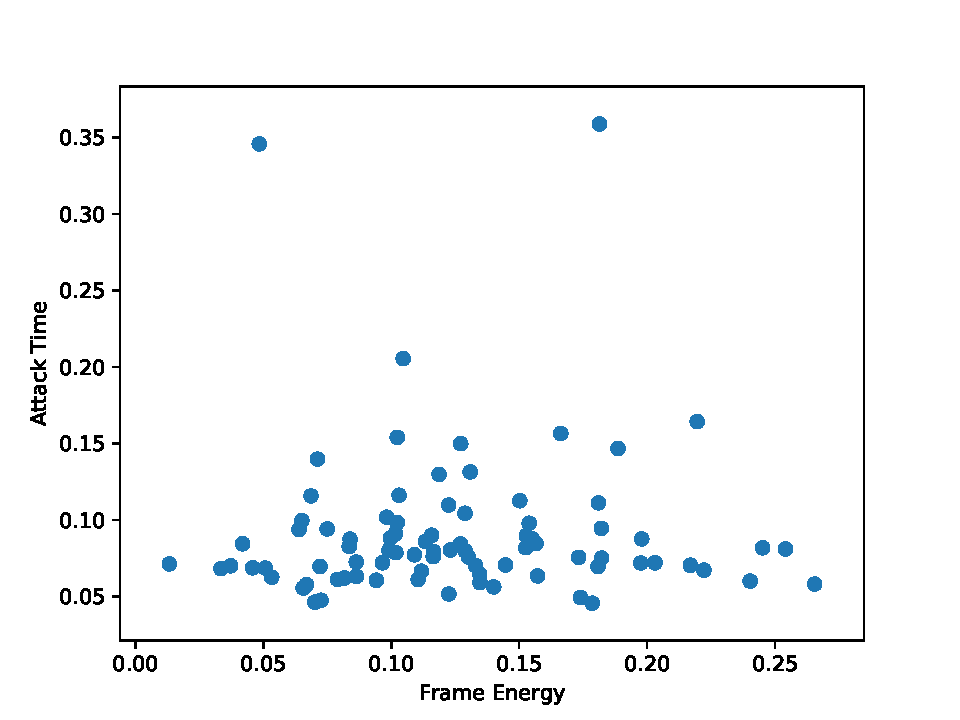
\includegraphics[width = 0.8\textwidth]{Figures/att.pdf}
    \caption{Attack Time über Frame Energy}
    \label{fig:attack_time}
\end{figure}

\begin{figure}[H]
    \center
    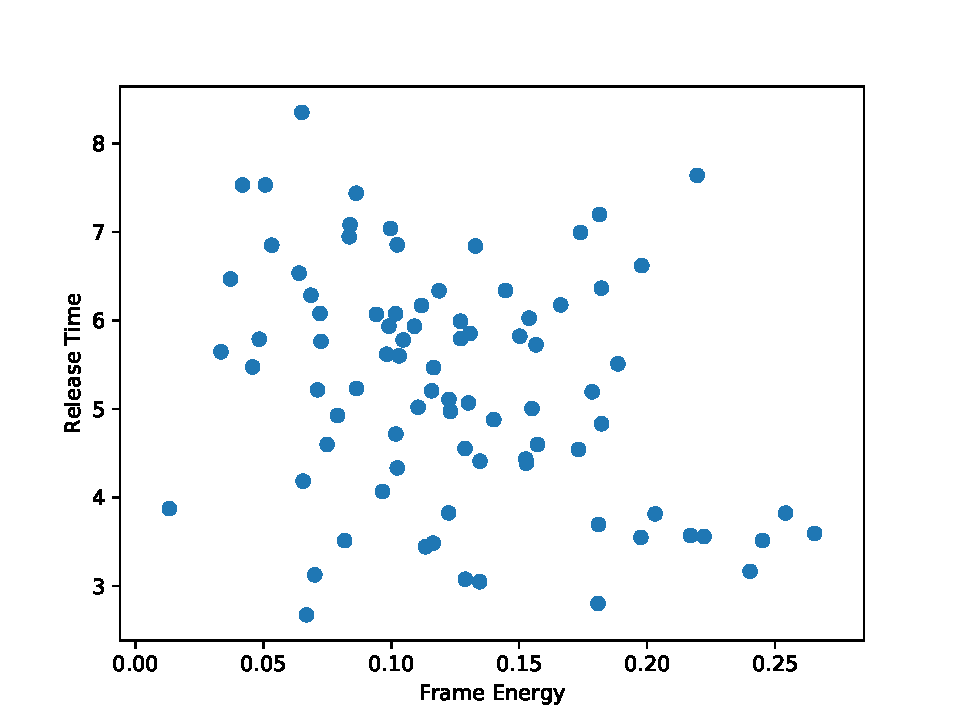
\includegraphics[width = 0.8\textwidth]{Figures/rel.pdf}
    \caption{Release Time über Frame Energy}
    \label{fig:release_time}
\end{figure}

\subsection{}
Für alle vier betrachteten Features haben wir in jeweiliger Kombination mit dem Feature Frame Energy ein Aufteilung in zwei Klassen mithilfe des \texttt{kmeans} Algorithmus durchgeführt.
Die Ergebnisse hiervon sind in den Abbildungen \ref{fig:harmonic_energy_c} bis \ref{fig:release_time_c} zu sehen.

\begin{figure}[H]
    \center
    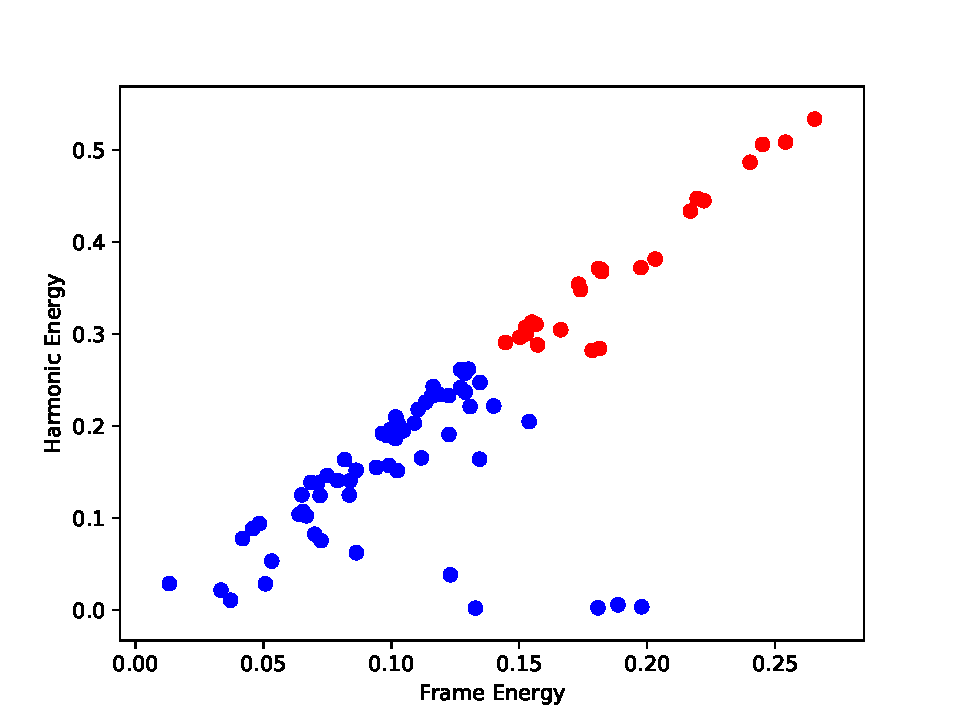
\includegraphics[width = 0.8\textwidth]{Figures/harmonic_energy_c}
    \caption{Harmonic Energy über Frame Energy mit Clustering }
    \label{fig:harmonic_energy_c}
\end{figure}


\begin{figure}[H]
    \center
    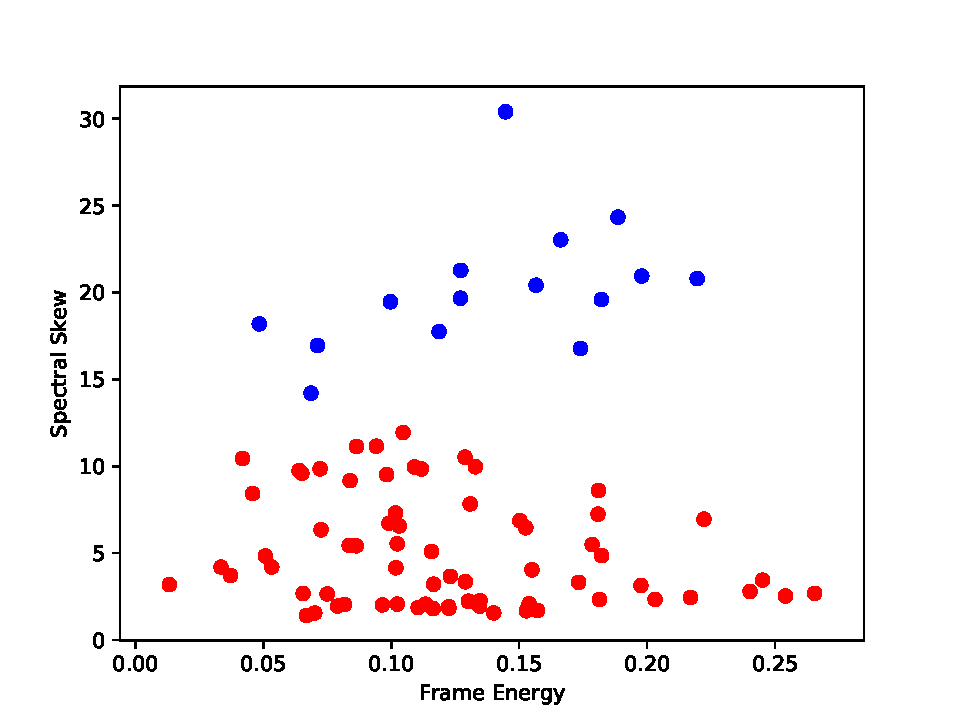
\includegraphics[width = 0.8\textwidth]{Figures/spectral_skew_c}
    \caption{Spectral Skew über Frame Energy mit Clustering }
    \label{fig:spectral_skew_c}
\end{figure}

\begin{figure}[H]
    \center
    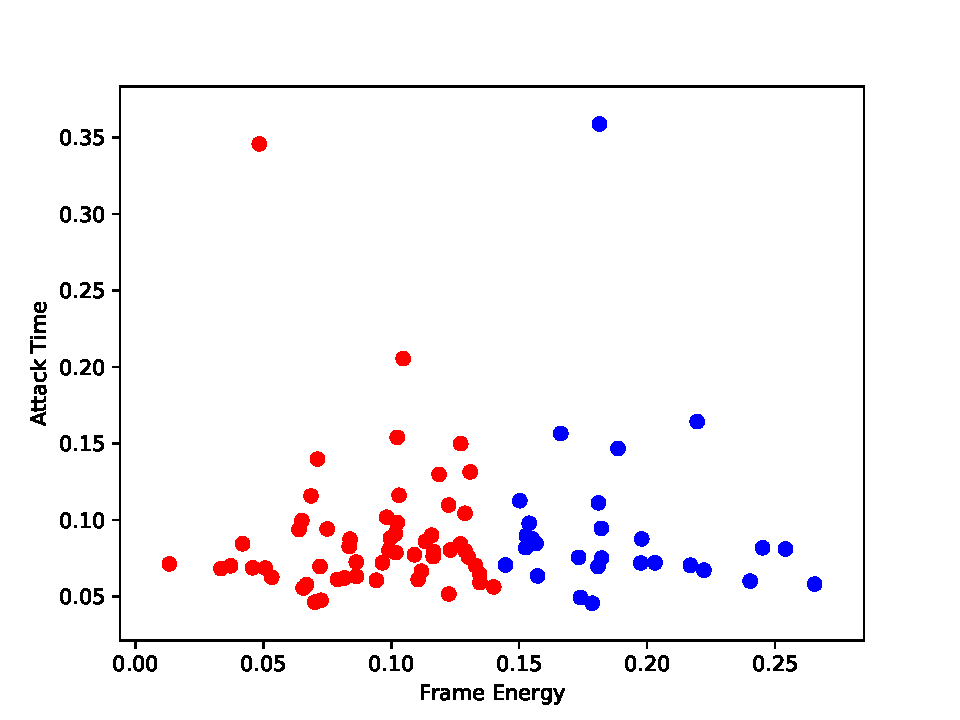
\includegraphics[width = 0.8\textwidth]{Figures/attack_time_c}
    \caption{Attack Time über Frame Energy mit Clustering }
    \label{fig:attack_time_c}
\end{figure}

\begin{figure}[H]
    \center
    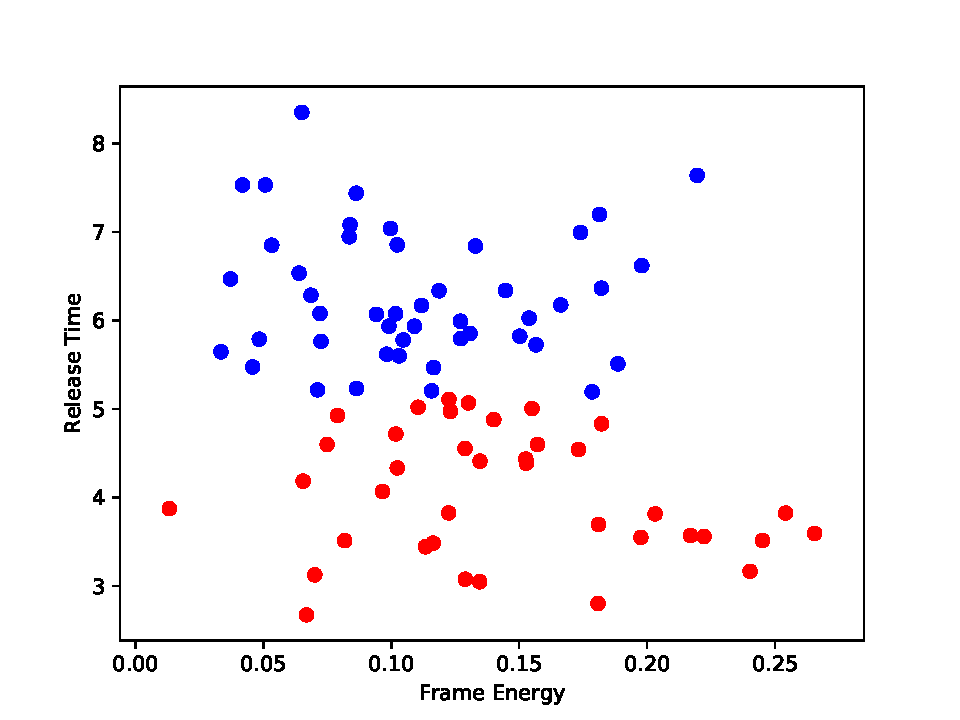
\includegraphics[width = 0.8\textwidth]{Figures/release_time_c.pdf}
    \caption{Release Time über Frame Energy mit Clustering}
    \label{fig:release_time_c}
\end{figure}

\subsection{}

Da die Harmonic Energy, der einzige Deskriptor ist, bei dem unsere theoretische Überlegung mit unserem als Referenz bzw. Ground Truth auserkorenen Deskriptor Frame Energy im Einklang steht, wählen wir auch dieses Merkmal um die Violinentöne endgültig in \textit{pp} für leise und \textit{ff} für laut zu klassifizieren. 
Die Ergebnisse unseres Clusterings sind in Tabelle \ref{tab:T} zu sehen.
Des weiteren ist in Abbildung \ref{fig:harmonic_energy_c_l} ein mit den Labels \textit{pp} und \textit{ff} versehener Scatterplot für Harmonic Energy und Frame Energy dargestellt.

\begin{figure}[H]
    \center
    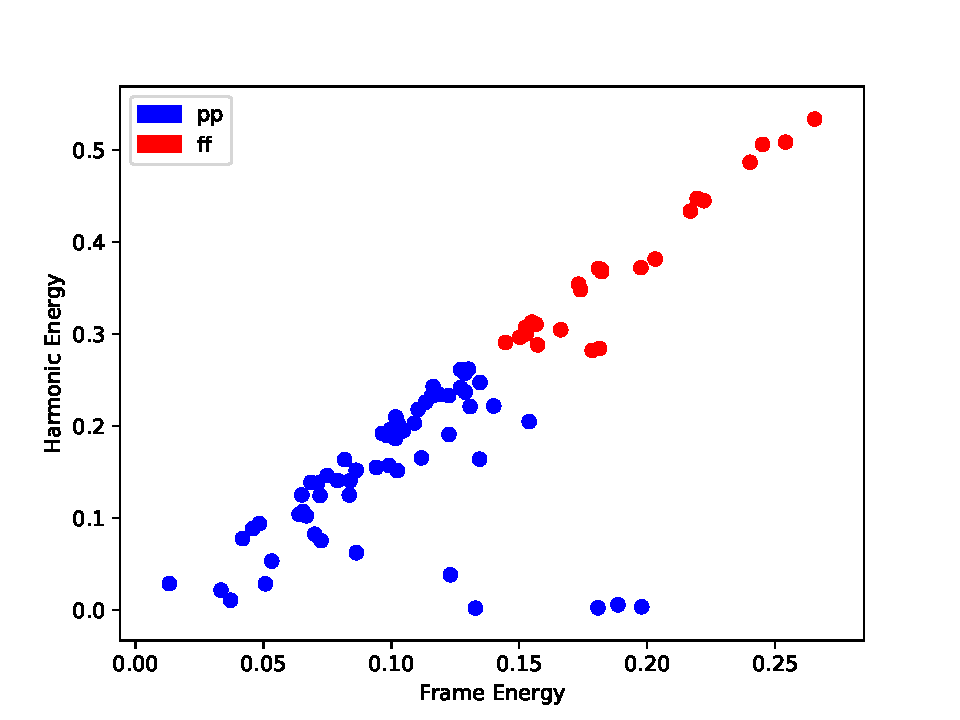
\includegraphics[width = 0.8\textwidth]{Figures/harmonic_energy_c_l}
    \caption{Harmonic Energy über Frame Energy mit Clustering und Labels \textit{pp} und \textit{ff} für leise uns laut}
    \label{fig:harmonic_energy_c_l}
\end{figure}

\begin{table}[H]
\centering
\caption{Klassifizierung der Audiodateien}
\label{tab:T}

\hfill
\begin{minipage}[b]{0.4\textwidth}
  \begin{tabular}{ | c | c | }
    \hline
    Dateiname & Klasse \\
    \hline
    SampLib\_BuK\_92\_441.wav & pp \\
    \hline
    SampLib\_BuK\_241\_441.wav & pp \\
    \hline
    SampLib\_BuK\_100\_441.wav & ff \\
    \hline
    SampLib\_BuK\_84\_441.wav & ff \\
    \hline
    SampLib\_BuK\_28\_441.wav & pp \\
    \hline
    SampLib\_BuK\_244\_441.wav & pp \\
    \hline
    SampLib\_BuK\_217\_441.wav & pp \\
    \hline
    SampLib\_BuK\_172\_441.wav & ff \\
    \hline
    SampLib\_BuK\_25\_441.wav & ff \\
    \hline
    SampLib\_BuK\_300\_441.wav & pp \\
    \hline
    SampLib\_BuK\_116\_441.wav & pp \\
    \hline
    SampLib\_BuK\_316\_441.wav & pp \\
    \hline
    SampLib\_BuK\_308\_441.wav & pp \\
    \hline
    SampLib\_BuK\_332\_441.wav & pp \\
    \hline
    SampLib\_BuK\_20\_441.wav & ff \\
    \hline
    SampLib\_BuK\_113\_441.wav & pp \\
    \hline
    SampLib\_BuK\_276\_441.wav & pp \\
    \hline
    SampLib\_BuK\_204\_441.wav & ff \\
    \hline
    SampLib\_BuK\_196\_441.wav & pp \\
    \hline
    SampLib\_BuK\_65\_441.wav & ff \\
    \hline
    SampLib\_BuK\_121\_441.wav & pp \\
    \hline
    SampLib\_BuK\_252\_441.wav & pp \\
    \hline
    SampLib\_BuK\_220\_441.wav & pp \\
    \hline
    SampLib\_BuK\_257\_441.wav & pp \\
    \hline
    SampLib\_BuK\_129\_441.wav & pp \\
    \hline
    SampLib\_BuK\_68\_441.wav & pp \\
    \hline
    SampLib\_BuK\_225\_441.wav & pp \\
    \hline
    SampLib\_BuK\_185\_441.wav & pp \\
    \hline
    SampLib\_BuK\_177\_441.wav & pp \\
    \hline
    SampLib\_BuK\_212\_441.wav & ff \\
    \hline
    SampLib\_BuK\_145\_441.wav & pp \\
    \hline
    SampLib\_BuK\_228\_441.wav & pp \\
    \hline
    SampLib\_BuK\_01\_441.wav & pp \\
    \hline
    SampLib\_BuK\_292\_441.wav & pp \\
    \hline
    SampLib\_BuK\_265\_441.wav & pp \\
    \hline
    SampLib\_BuK\_57\_441.wav & pp \\
    \hline
    SampLib\_BuK\_153\_441.wav & ff \\
    \hline
    SampLib\_BuK\_268\_441.wav & pp \\
    \hline
    SampLib\_BuK\_41\_441.wav & pp \\
    \hline
    SampLib\_BuK\_140\_441.wav & pp \\
    \hline
    SampLib\_BuK\_49\_441.wav & pp \\
    \hline
    SampLib\_BuK\_180\_441.wav & pp \\
    \hline
  \end{tabular}
\end{minipage}
\hfill
\begin{minipage}[b]{0.4\textwidth}
  \begin{tabular}{ | c | c | }
    \hline
    Dateiname & Klasse \\
    \hline
    SampLib\_BuK\_233\_441.wav & pp \\
    \hline
    SampLib\_BuK\_164\_441.wav & pp \\
    \hline
    SampLib\_BuK\_201\_441.wav & pp \\
    \hline
    SampLib\_BuK\_297\_441.wav & pp \\
    \hline
    SampLib\_BuK\_89\_441.wav & pp \\
    \hline
    SampLib\_BuK\_137\_441.wav & pp \\
    \hline
    SampLib\_BuK\_36\_441.wav & pp \\
    \hline
    SampLib\_BuK\_124\_441.wav & ff \\
    \hline
    SampLib\_BuK\_12\_441.wav & pp \\
    \hline
    SampLib\_BuK\_04\_441.wav & pp \\
    \hline
    SampLib\_BuK\_273\_441.wav & ff \\
    \hline
    SampLib\_BuK\_281\_441.wav & pp \\
    \hline
    SampLib\_BuK\_188\_441.wav & ff \\
    \hline
    SampLib\_BuK\_249\_441.wav & pp \\
    \hline
    SampLib\_BuK\_60\_441.wav & ff \\
    \hline
    SampLib\_BuK\_305\_441.wav & pp \\
    \hline
    SampLib\_BuK\_132\_441.wav & pp \\
    \hline
    SampLib\_BuK\_09\_441.wav & pp \\
    \hline
    SampLib\_BuK\_169\_441.wav & pp \\
    \hline
    SampLib\_BuK\_81\_441.wav & ff \\
    \hline
    SampLib\_BuK\_284\_441.wav & ff \\
    \hline
    SampLib\_BuK\_236\_441.wav & ff \\
    \hline
    SampLib\_BuK\_44\_441.wav & pp \\
    \hline
    SampLib\_BuK\_76\_441.wav & ff \\
    \hline
    SampLib\_BuK\_17\_441.wav & pp \\
    \hline
    SampLib\_BuK\_289\_441.wav & pp \\
    \hline
    SampLib\_BuK\_313\_441.wav & pp \\
    \hline
    SampLib\_BuK\_52\_441.wav & ff \\
    \hline
    SampLib\_BuK\_97\_441.wav & ff \\
    \hline
    SampLib\_BuK\_321\_441.wav & ff \\
    \hline
    SampLib\_BuK\_33\_441.wav & pp \\
    \hline
    SampLib\_BuK\_209\_441.wav & pp \\
    \hline
    SampLib\_BuK\_324\_441.wav & pp \\
    \hline
    SampLib\_BuK\_105\_441.wav & pp \\
    \hline
    SampLib\_BuK\_161\_441.wav & pp \\
    \hline
    SampLib\_BuK\_260\_441.wav & ff \\
    \hline
    SampLib\_BuK\_329\_441.wav & pp \\
    \hline
    SampLib\_BuK\_193\_441.wav & pp \\
    \hline
    SampLib\_BuK\_156\_441.wav & ff \\
    \hline
    SampLib\_BuK\_73\_441.wav & ff \\
    \hline
    SampLib\_BuK\_108\_441.wav & pp \\
    \hline
    SampLib\_BuK\_148\_441.wav & ff \\
    \hline
    \end{tabular}
  \end{minipage}

\hfill
\end{table}



